\section{Theorie}
\label{sec:Theorie}

Einer elektromagnetischem Welle kann ein Poynting-Vektor zu geordnet werden. Der Betrag wird als 
\begin{equation}
    \left| \vec{S}\right|  = v \epsilon \epsilon_0  \vec{E}²
    \label{eq:betragpoynting}
\end{equation}
 geschrieben werden.

Trifft eine ebene Lichtwelle unter dem Winkel  $\alpha$  aus dem Vakuum auf eine Grenzfläche zu einem anderen Medium, so wird ein Teil der Strahlung gebrochen $\vec{E_r}$ und der andere reflektiert $\vec{E_d}$. Es wird angenommen, dass kein Licht vom Medium absorbiert wird.


\begin{figure}
    \centering
    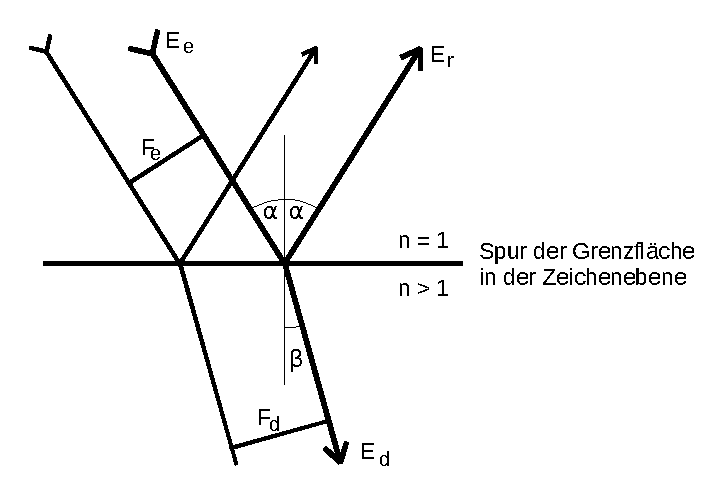
\includegraphics{Brechung an einer Ebene.pdf}
    \caption{Brechung an einer Ebene.} 
    \label{fig:abb1}
\end{figure}

Wie in der oberen Grafik \ref{fig:abb1} zu sehen ist, ist der Brechungswinkel $ \beta$ kleiner als der Brechungswinkel $\alpha$, da das Licht im Medium eine geringere Geschwindigkeit hat als im Vakuum.
Daraus bedingt sich eine Querschnittsänderung der einlaufenden Strahlung von $F_e$ auf $F_d$. 
Es gilt die Energieerhaltung, die sich als
\begin{equation}
    S_e F_e = S_r F_e +  S_d F_d
    \label{eq:Energieerhaltung}
\end{equation}
oder auch 

\begin{equation}
    S_e \cos(\alpha) = S_r \cos(\alpha) +  S_d \cos(\beta)
    \label{eq:Energieerhaltungwinkel}
\end{equation}
schreiben lässt.
Die Gleichung \eqref{eq:Energieerhaltungwinkel} lässt sich mit hilfe der Gleichung \eqref{eq:betragpoynting} für die Poynting-Vektoren zu 
\begin{equation}
    c \epsilon_0 \vec{E_e}² \cos(\alpha) = c \epsilon_0 \vec{E_r}^2 \cos(\alpha) + v \epsilon \epsilon_0 \vec(E_d)^2 \cos(\beta)
    \label{eq:eins}
\end{equation}
umstellen. Der Brechungsindex ist das Verhältnis zwischen der Lichtgeschwindigkeit im Vakuum und der im Medium 
\begin{equation}
    n = \dfrac{c}{v} ,
    \label{eq:Brechungsindex}
\end{equation}
damit kann anstelle der Gleichung \eqref{eq:eins} auch 
\begin{equation}
    (\vec{E_e}^2  - \vec{E_r}^2)n \cos(\alpha) = \epsilon \vec(E_d)^2 \cos(\beta)
    \label{eq:zwei}
\end{equation}
geschrieben werden.

Wenn die Maxwellsche Relation
\begin{equation*}
    n^2 = \epsilon
    \label{eq:Maxwellschrelation}
\end{equation*}
in die Gleichung \eqref{eq:zwei} eingesetzt wird, ergibt sich 
\begin{equation}
    (\vec{E_e}^2  - \vec{E_r}^2) \cos(\alpha) = n \vec(E_d)^2 \cos(\beta).
    \label{eq:drei}
\end{equation}

Die eingehende Welle, die durch den Vektor $\vec{E_e}$ gegeben ist, besteht aus einem parallel und senkrecht polarisierten Teil.
\begin{equation*}
    \vec{E_e} = \vec{E_\parallel}  + \vec{E_\perp}
    \label{eq:vier}
\end{equation*}
Die unterschiedlich polarisierten Teile der Welle verhalten sich an der Grenzfläche verschieden.
Aus diesem Grund ist es notwendig den parallelen und senkrechten Teil seperat zu betrachten. 
